\section{On-chain Protocol}\label{sec:on-chain}

\todo{Open problem: ensure abort is always possible. e.g. by individual aborts or undoing commits}
\todo{Open problem: ensure fanout is always possible, e.g. by limiting complexity of $U_0$}

The following sections describe the the \emph{on-chain} protocol controlling the
life-cycle of a Hydra head, which can be intuitively described as a state
machine (see Figure~\ref{fig:SM_states_basic}). Each transition in this state
machine is represented and caused by a corresponding Hydra protocol transaction
on-chain: $\mtxInit{}$, $\mtxCom{}$, $\mtxAbort{}$, $\mtxCollect{}$,
$\mtxClose{}$, $\mtxContest{}$, and $\mtxFanout{}$.

% TODO: Could include a combined overview, slightly more detailed than Figure 1
% of the transaction trace for the full life cycle maybe?

State machines in the EUTxO ledger model are commonly described using the
\emph{constraint emitting machine (CEM)} formalism~\cite{eutxo}, e.g.~the
original paper describes the Hydra Head protocol using this
notation~\cite{hydrahead20}. Although inspired by CEMs, this specification uses
a more direct representation of individual transactions to simplify description
of non-state-machine transactions and help translation to concrete
implementations on Cardano. The structure of the state machine is enforced
on-chain through \emph{scripts} which run as part of the ledger's validation of
a transaction (see Section~\ref{sec:eutxo}). For each protocol transaction, the
specification defines the structure of the transaction and enumerates the
transaction constraints enforced by the scripts ($\cemTxCon$ in the CEM
formalism). \\

\noindent The protocol defines one minting policy script and three validator scripts:
\begin{itemize}
	\item $\muHead$ governs minting of state and participation tokens in
	      $\mtxInit{}$ and burning of these tokens in $\mtxAbort{}$ and
	      $\mtxFanout{}$.
	\item $\nuInitial$ controls how UTxOs are committed to the head in
	      $\mtxCommit{}$ or when the head initialiazation is aborted via
	      $\mtxAbort{}$.
	\item $\nuCommit$ controls the collection of committed UTxOs into the head in
	      $\mtxCollect$ or that funds are reimbursed in an $\mtxAbort{}$.
	\item $\nuHead$ represents the main protocol state machine logic and ensures
	      contract continuity throughout $\mtxCollectCom{}$, $\mtxClose{}$,
	      $\mtxContest{}$ and $\mtxFanout{}$.
\end{itemize}

\subsection{Init transaction}\label{sec:init-tx}

The \mtxInit{} transaction creates a head instance and establishes the initial
state of the protocol and is shown in Figure~\ref{fig:initTx}. The head
instance is represented by the unique currency identifier $\cid$ created by
minting tokens using the $\muHead$ minting policy script which is parameterized
by $\seed \in \tyOutRef$:
\[
	\cid = \hash(\muHead(\seed))
\]

\begin{figure}
	\centering
	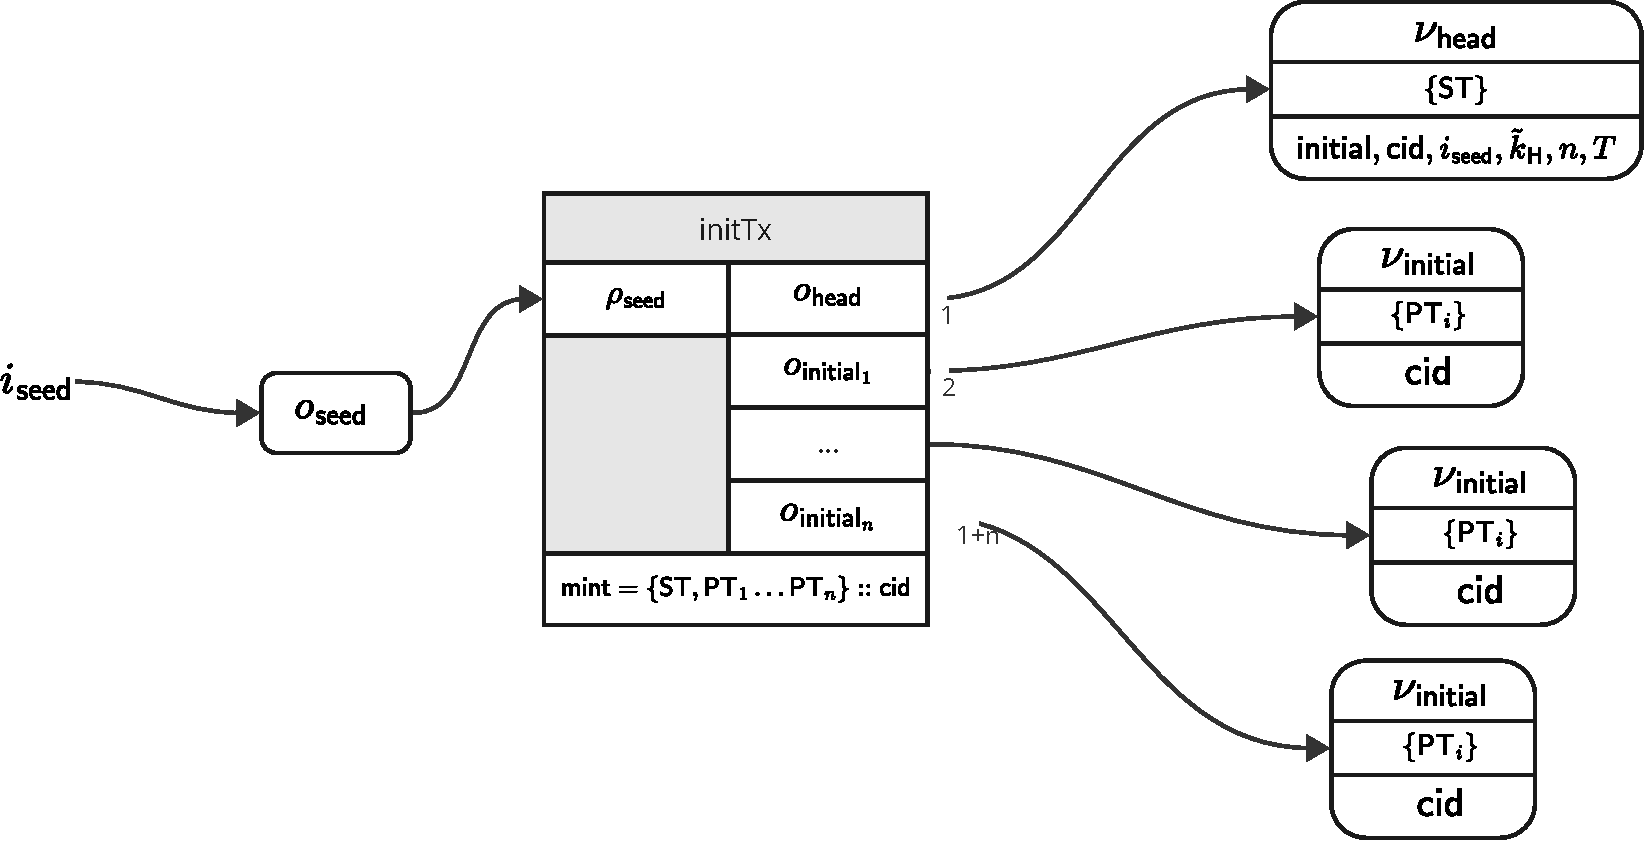
\includegraphics[width=0.8\textwidth]{figures/initTx.pdf}
	\caption{\mtxInit{} transaction spending a seed UTxO, and producing the head
		output in state $\stInitial$ and initial outputs for each participant.}\label{fig:initTx}
\end{figure}

\noindent Two kinds of tokens are minted:
\begin{itemize}
	\item A single \emph{State Thread (ST)} token marking the head output. This
	      output contains the state of the protocol on-chain and the token ensures
	      contract continuity. The token name is the well known string
	      \texttt{HydraHeadV1}, i.e.
	      $\st = \{\cid \mapsto \texttt{HydraHeadV1} \mapsto 1\}$.\todo{value
		      notation}
	\item One \emph{Participation Token (PT)} per participant
	      $i \in \{1 \dots \nop \}$ to be used for authenticating further
	      transactions and to ensure every participant can commit and cannot be
	      censored. The token name is the participant's verification key hash
	      $\keyHash_{i} = \hash(\msVK_{i})$ of the verification key as received
	      during protocol setup, i.e.
	      $\pt_{i} = \{\cid \mapsto \keyHash_{i} \mapsto 1\}$.
\end{itemize}

\noindent Consequently, the \mtxInit{} transaction

\begin{itemize}
	\item has at least input $\seed$,
	\item mints the state thread token $\st$, and one $\pt$ for each of the $\nop$
	      participants with policy $\cid$,
	\item has $\nop$ initial outputs
	      $o_{\mathsf{initial}_{i}} = (\valInitial{i}, \nuInitial, \datumInitial{})$,
	      where $\datumInitial{} = \cid$,
	\item has one state machine output
	      $o_{\mathsf{head}} = (\valHead, \nuHead, \datumHead)$. The initial state
	      of the protocol is captured by the datum
	      \[
		      \datumHead = (\stInitial,\cid',\seed',\hydraKeysAgg,\nop,\cPer)
	      \]
	      where
	      \begin{mitemize}
		      \item $\stInitial$ is a state identifier,
		      \item $\cid'$ is the unique currency id of this instance,
		      \item $\seed'$ is the seed input parameter of $\muHead$,
		      \item $\hydraKeysAgg$ is the aggregated off-chain multi-signature key established during the
		      setup phase,
		      \item $\nop$ is the number of head participants, and
		      \item $\cPer$ is the length of the contestation period.
	      \end{mitemize}
\end{itemize}

\noindent The $\muHead(\seed)$ minting policy is the only script that verifies
init transactions by checking and can be redeemed with either a
$\mathsf{Mint}$ or $\mathsf{Burn}$ redeemer:
\begin{itemize}
	\item When minting via the $\mathsf{Mint}$ redeemer,
	      \begin{enumerate}
		      \item The seed output is spent in this transaction. This guarantees uniqueness of the policy $\cid$ because the EUTxO ledger ensures that $\seed$ cannot be spent twice in the same chain.
		            $(\seed, \cdot) \in \txInputs$
		      \item \textcolor{blue}{Right number of unique tokens are minted
			            $|\{\cid \mapsto \cdot \mapsto 1\} \in \txMint| = \nop + 1$}
		            % TODO: different than in GDoc
		      \item State token is sent to the head validator $\st \in \valHead$
		      \item \textcolor{blue}{Correct number of initial outputs $|(\cdot, \nuInitial, \cdot) \in \txOutputs| = n$}
		            % TODO: different than in GDoc
		      \item All initial outputs hold a participation token $\forall i \in [1 \dots n] : \{\cid \mapsto \cdot \mapsto 1\} \in \valInitial{i}$
		      \item The $\datum_{\mathsf{head}}$ contains own currency id $\cid = \cid'$ and the right seed reference $\seed = \seed'$.
	      \end{enumerate}
	\item When burning via the $\mathsf{Burn}$ redeemer,
	      \begin{enumerate}
		      \item All tokens in $\txMint$ need to be of negative quantity
		            $\forall \{\cid \mapsto \cdot \mapsto q\} \in \txMint : q < 0$.
	      \end{enumerate}
\end{itemize}

\noindent \textbf{Important:} The $\muHead$ minting policy only ensures
uniqueness of $\cid$, that the right amount of tokens have been minted and sent
to $\nuHead$ and $\nuInitial$ respectively, while these validators in turn
ensure continuity of the contract. However, it is \textbf{crucial} that all head
members check that any head output contains a token of policy $\cid$ which
satisfies $\cid = \hash(\muHead(\seed))$. The
$\seed$ from a head datum can be used to determine this.
Also, head members likely want to check
whether the right participants have gotten PTs and the initial state is
consistent with parameters agreed during setup. See the initialTx behavior in
Figure~\ref{fig:off-chain-prot} for details about these checks.\\

\subsection{Commit Transaction}\label{sec:commit-tx}

A \mtxCom{} transaction may be submitted by each participant
$\forall i \in \{1 \dots \nop\}$ and is depicted on the right hand side of
Figure~\ref{fig:commitTx}. It has the following structure:
\begin{itemize}
	\item One input $i_{\mathsf{initial}} = (\txOutRef_{\mathsf{initial}}, \redeemerInitial{})$
	      spending $o_{\mathsf{initial}} = (\valInitial{}, \nuInitial, \datumInitial{})$
	\item Zero or one input with reference
	      $\txOutRef_{\mathsf{committed}}$ spending output
	      $o_{\mathsf{committed}} = (\val_{\mathsf{committed}}, \cdot , \cdot)$
	\item One output $o_{\mathsf{commit}} = (\valCommit{}, \nuCommit, \datumCommit{})$
\end{itemize}

\noindent The $\nuInitial$ validator with $\datumInitial{} = \cid$ and $\redeemerInitial{} = \txOutRef_{\mathsf{committed}}$ ensures that:
\begin{menumerate}
	\item The committed value is in the output $\valCommit{} = \valInitial{} \cup \val_{\mathsf{committed}}$
	\item The currency id and committed output are recorded in the output datum
	$\datumCommit{} = (\cid, U_{i})$ where\todo{rename $U_{i}$ to $C_{i}$}
	$U_{i} = (\txOutRef_{\mathsf{committed}},\bytes(o_{\mathsf{committed}}))$
	\item Transaction is signed by a participant $\exists \{\cid \mapsto \keyHash_{i} \mapsto 1\} \in \valCommit{} \Rightarrow \keyHash_{i} \in \txKeys$
	\item No minting or burning  $\txMint = \varnothing$
\end{menumerate}

\noindent The $\nuCommit$ validator ensures the output is collected by either a \mtxCCom{} in Section~\ref{sec:collect-tx} or \mtxAbort{} in Section~\ref{sec:abort-tx} transaction of the on-chain state machine, selected by the appropriate redeemer.

\begin{figure}[h]
	\centering
	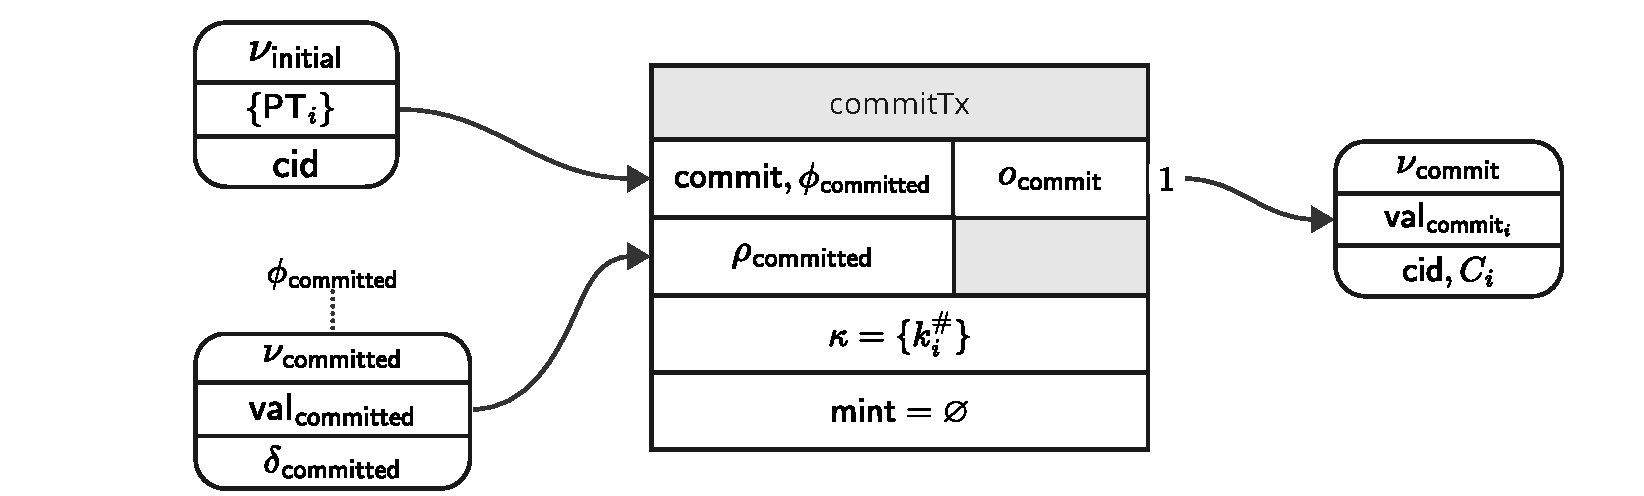
\includegraphics[width=0.8\textwidth]{figures/commitTx.pdf}
	\caption{\mtxCom{} transaction spending an initial output and a single
		committed output, and producing a commit output.}\label{fig:commitTx}
\end{figure}

\subsection{CollectCom Transaction}\label{sec:collect-tx}

\noindent The \mtxCCom{} transaction (Figure~\ref{fig:collectComTx}) collects all the committed UTxOs to the same head. It has
\begin{itemize}
	\item one input spending from $\nuHead$ holding the $\st$, and
	\item $\forall i \in \{1 \dots \nop\}$ inputs spending \mtxCom{} outputs $(\valCommit{i}, \nuCommit, \datumCommit{i})$ with $\pt_{i} \in \valCommit{i}$ and $\datumCommit{i} = (\cid, U_{i})$.
\end{itemize}

\noindent The input spending from and paying to the $\nuHead$ validator, checks the state
of the CEM is advanced:
\[
	(\stInitial,\cid,\seed,\hydraKeysAgg,\nop,\cPer) \xrightarrow{\stCollect} (\stOpen,\cid,\hydraKeysAgg,\nop,\cPer,\eta)
\]

\begin{samepage}
	\noindent Furthermore, $\nuHead$ checks these constraints:
	\begin{menumerate}
		\item Collect commits in $\eta = (0, U^{\#})$, where
		$U^{\#} = \combine([U_{1}, \dots, U_{\nop}])$:
		\[
			\combine(\underline{U}) = \hash(\mathsf{concat}({\sortOn(1, \underline{U})}^{\downarrow2}))
		\]
		\todo{Limit size of what we can collect (likely by bytes)}\todo{also mention in off-chain protocol}
		That is, given a list of commits $\underline{U}$, where each element is a pair
		of an $\txOutRef$ and the serialised representation of what was committed
		$U_{i} \in (\tyOutRef \times \tyBytes)$, $\combine$ sorts this list by the
		$\txOutRef$, concatenates all the bytes and hashes the
		result\footnote{Sorting is required to ensure a canonical representation
			which can also be reproduced from the UTxO set later in the fanout.}.

		\item All committed value captured and no additional funds ``enter'' or ``leave''\\
		$\val' = \mathsf{ST} \cup (\bigcup_{i=1}^{n} \valCommit{i})$
		\item Every participant had the chance to commit, by checking all tokens are present in output\footnote{This is sufficient as a Head participant would check off-chain whether a Head is initialized correctly with the right number of tokens.}
		$|\{\cid \rightarrow . \rightarrow 1\} \in \val'| = \nop + 1$
		\item Transaction is signed by a participant $\exists \{\cid \mapsto \keyHash_{i} \mapsto 1\} \in \valCommit{} \Rightarrow \keyHash_{i} \in \txKeys$\todo{allow anyone to do this?}
		\item No minting or burning  $\txMint = \varnothing$
	\end{menumerate}
\end{samepage}

\noindent Each spent $\nuCommit$ validator with $\datumCommit{i} = (\cid,\cdot)$ and $\redeemerCommit{i} = \mathsf{Collect}$ ensures that:
\begin{menumerate}
	\item The state token of currency $\cid$ is present in the output value
	$\{\st \mapsto 1\} \in \val'$.
\end{menumerate}

\begin{figure}[h]
	\centering
	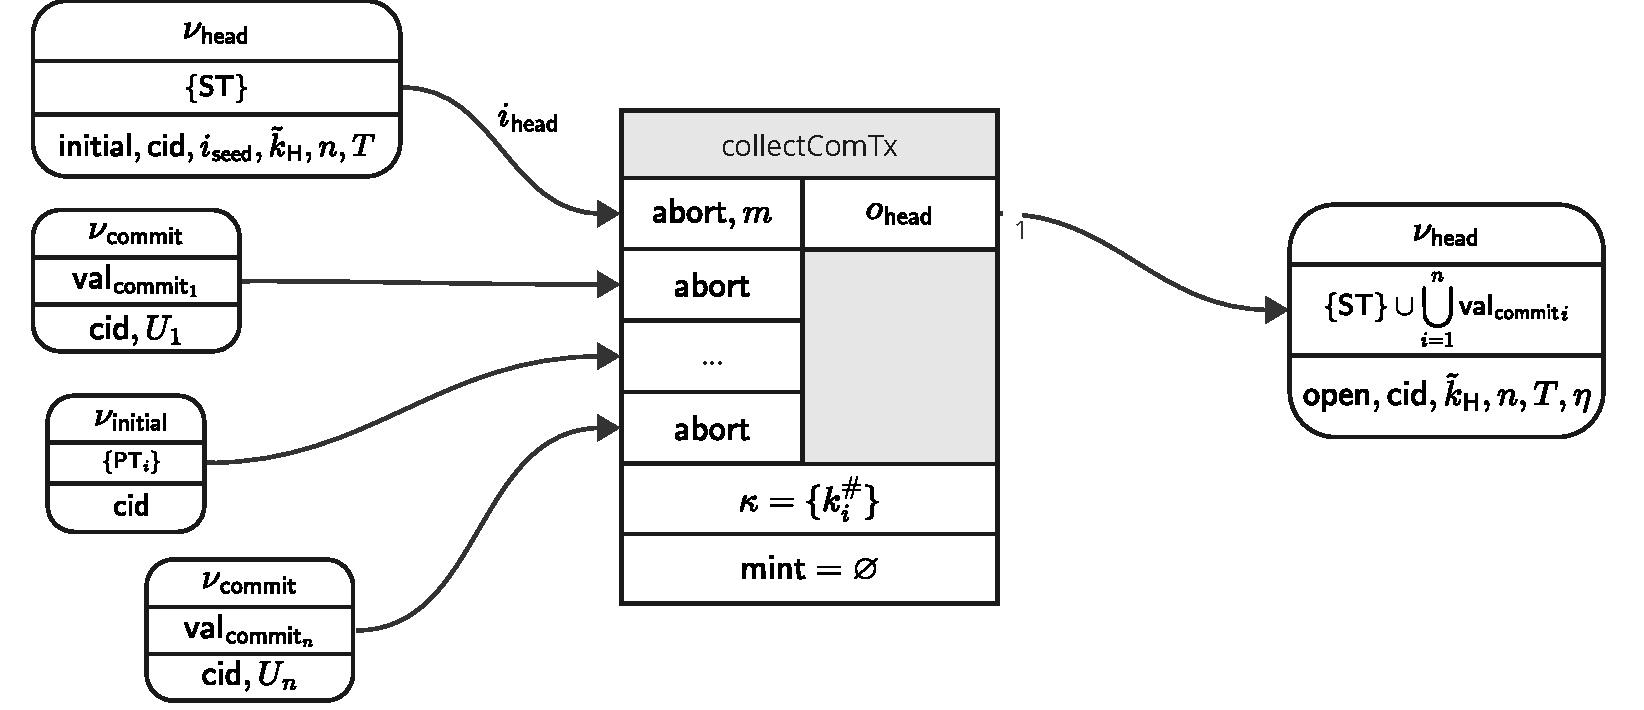
\includegraphics[width=0.8\textwidth]{figures/collectComTx.pdf}
	\caption{\mtxCCom{} transaction spending the head output in $\stInitial$
		state and collecting from multiple commit outputs into a single
		$\stOpen$ head output.}\label{fig:collectComTx}
\end{figure}

\subsection{Abort Transaction}\label{sec:abort-tx}

\begin{samepage}
	The \mtxAbort{} transaction (see Figure~\ref{fig:abortTx}) allows a
	party to abort the creation of a head and consists of
	\begin{itemize}
		\item one input spending from $\nuHead$ holding the $\st$, and
		\item $\forall i \in \{1 \dots \nop\}$ inputs either
		      \begin{itemize}
			      \item spending from an initial output $(\valInitial{i}, \nuInitial, \cid)$ with $\pt_{i} \in \valInitial{i}$, or
			      \item spending from a commit output $(\valCommit{i}, \nuCommit, \datumCommit{i})$ with $\pt_{i} \in \valCommit{i}$,
		      \end{itemize}
		\item $m$ outputs to redistribute already committed UTxOs.
	\end{itemize}
\end{samepage}

\noindent Note that \mtxAbort{} represents a final transition of the CEM and hence there
is no state machine output. The input spending from $\nuHead$ does provide the
number of reimbursed outputs $m$ as redeemer \todo{m is implicit, not required as redeemer} and checks the state of the CEM is
advanced to the final $\stFinal$ as follows:

\[
	(\stInitial,\cid,\seed,\hydraKeysAgg,\nop,\cPer) \xrightarrow[m]{\stAbort} \stFinal.
\]

\begin{samepage}
	\noindent The $\nuHead$ validator ensures that:
	\begin{menumerate}
		\item All UTxOs committed into the head are reimbursed exactly as they were
		committed. By comparing hashes of serialised representations of the $m$
		reimbursing outputs\footnote{Only the first $m$ outputs are used for
			reimbursing, while more outputs may be present in the transaction, e.g for
			change} and canonically combined committed UTxOs $U_{i}$ where $(\cdot, U_{i}) = \datum_{commit_{i}}$ from \mtxCom{}~\ref{sec:commit-tx}:
		\todo{list/tuple comprehensions?}
		\[
			\hash(\bigoplus_{j=1}^{m} \bytes(\txOutputs[j])) = \combine([U_{i} ~ | ~ \forall [1\dots\nop], U_{i} \neq \bot])
		\]

		\item Transaction is signed by a participant $\exists \{\cid \mapsto \keyHash_{i} \mapsto -1\} \in \txMint \Rightarrow \keyHash_{i} \in \txKeys$
		\item All tokens are burnt
		$|\{\cid \mapsto \cdot \mapsto -1\} \in \txMint| = \nop + 1$
	\end{menumerate}
\end{samepage}

\noindent Each spent $\nuInitial$ validator with $\datumInitial{i} = \cid$ and $\redeemerInitial{i} = \mathsf{Abort}$ ensures that:
\begin{menumerate}
	\item The state token of currency $\cid$ is getting burned $\{\st \mapsto -1\} \subseteq \txMint$.
\end{menumerate}

\noindent Each spent $\nuCommit$ validator with $\datumCommit{i} = (\cid,\cdot)$ and $\redeemerCommit{i} = \mathsf{Abort}$ ensures that:
\begin{menumerate}
	\item The state token of currency $\cid$ is getting burned $\{\st \mapsto -1\} \subseteq \txMint$.
\end{menumerate}

\begin{figure}[h]
	\centering
	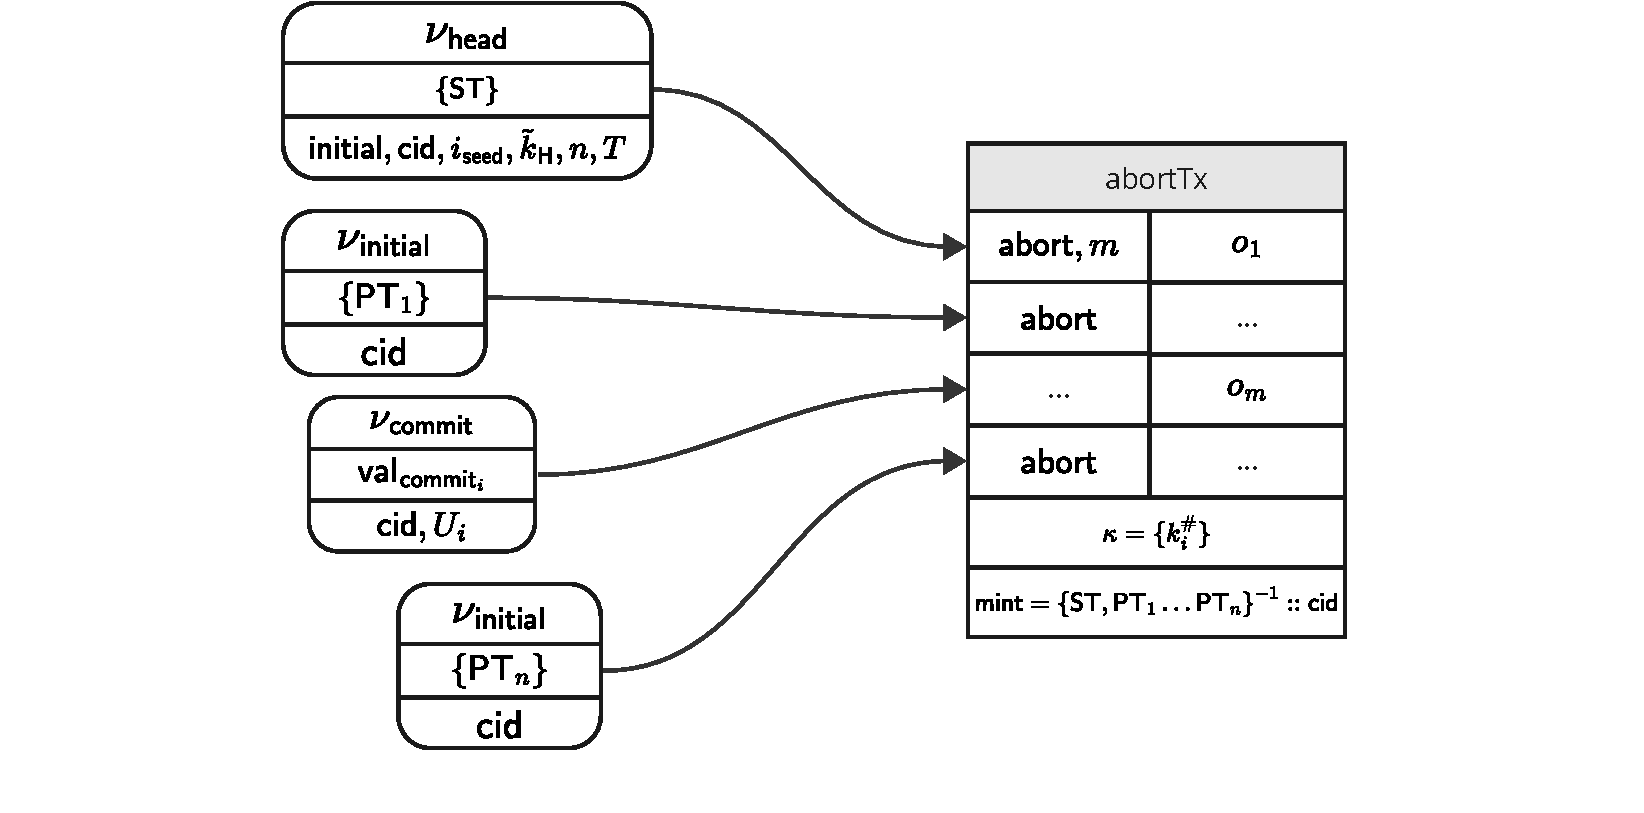
\includegraphics[width=0.8\textwidth]{figures/abortTx.pdf}
	\caption{\mtxAbort{} transaction spending the $\stInitial$ state head
		output and collecting all initial and commit outputs, which get reimbursed
		by outputs $o_{1} \dots o_{n}$. Note that each $\pt$ may be in either, an
		initial or commit output.}\label{fig:abortTx}
\end{figure}

\subsection{Close Transaction}\label{sec:close-tx}

In order to close a head, a head member may post the \mtxClose{} transaction
(see Figure~\ref{fig:closeTx}). This transaction has a single input
spending from the $\nuHead$ and paying to the $\nuHead$ validator, which checks
the state of the CEM is advanced:
\[
	(\stOpen,\cid,\hydraKeysAgg,\nop,\cPer,\eta) \xrightarrow[\xi]{\stClose} (\stClosed,\cid,\hydraKeysAgg,\nop,\cPer,\eta_0,\eta',\contesters,\Tfinal)
\]

\begin{samepage}
	\noindent The $\nuHead$ validator performs these checks:
	\begin{enumerate}
		\item Recorded the initial snapshot state\footnote{Needed to make off-chain signatures replay resistant, see~\ref{sec:rollbacks} for details.} $\eta_0 = \eta$
		\item New snapshot state $(s', \cdot) = \eta'$ is the initial $\eta_{0}$
		      or correctly signed by all participants in multi-signature $\xi$ \\
		      \[
			      \left\{\begin{array}{ll}
				      \msVfy(\hydraKeysAgg,(\cid || \eta_{0} || \eta'),\xi) = \true & \mathrm{if} ~ s' > 0, \\
				      \eta' = \eta_{0}                                              & \mathrm{otherwise}
			      \end{array}\right.
		      \]
		\item Initialize the set of contesters\footnote{Allows the closing party
			      to also contest and is required for use cases where pre-signed, valid in
			      the future, close transactions are used to delegate head closing.}
		      $\contesters = \emptyset$
		\item Correct contestation deadline $\Tfinal = \txValidityMax + T$ \todo{Add "parameters not change" constraint}
		\item Bounded confirmation window\footnote{Ensures head $\Tfinal$ is at most
			      $2*T$ in the future.} $\txValidityMax - \txValidityMin \leq T$
		\item Value in the head is preserved $\val' = \val$
		\item Transaction is signed by a participant $\exists \{\cid \mapsto \keyHash_{i} \mapsto 1\} \in \val' \Rightarrow \keyHash_{i} \in \txKeys$
		\item No minting or burning $\txMint = \varnothing$
	\end{enumerate}
\end{samepage}

\begin{figure}[h]
	\centering
	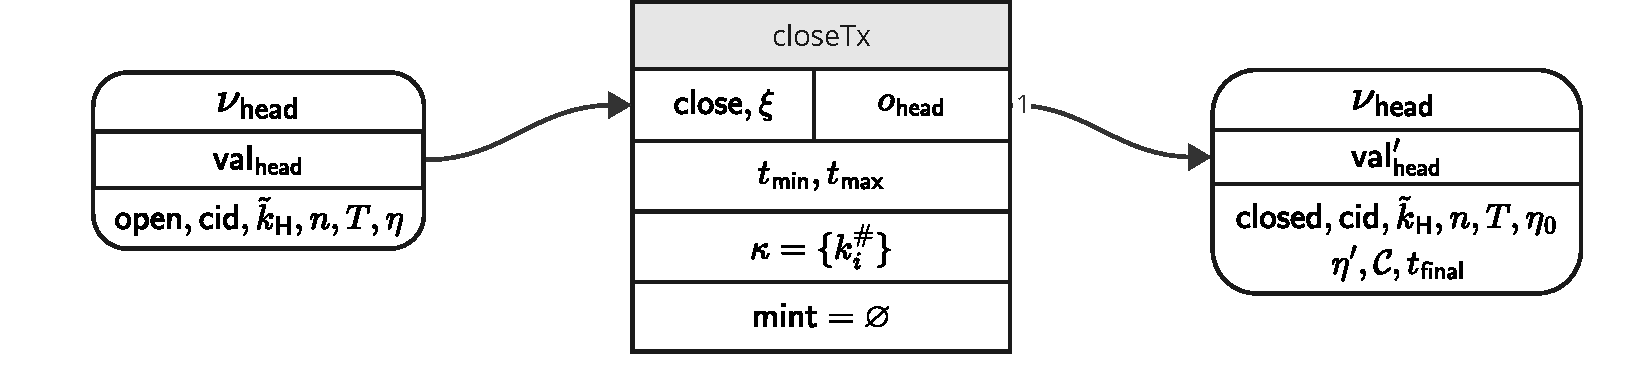
\includegraphics[width=0.8\textwidth]{figures/closeTx.pdf}
	\caption{\mtxClose{} transaction spending the $\stOpen$ head output and producing a $\stClosed$ head output.}\label{fig:closeTx}
\end{figure}

\subsection{Contest Transaction}\label{sec:contest-tx}

The \mtxContest{} transaction (see Figure~\ref{fig:contestTx}) is posted
by a party to prove the currently $\stClosed$ state is not the latest one. This
transaction has a single input spending from the $\nuHead$ and paying to the
$\nuHead$ validator, which checks the state of the CEM is advanced:
\[
	(\stClosed,\cid,\hydraKeysAgg,\nop,\cPer,\eta_0,\eta,\contesters,\Tfinal) \xrightarrow[\xi]{\stContest} (\stClosed,\cid,\hydraKeysAgg,\nop,\cPer,\eta_0,\eta',\contesters',\Tfinal')
\]

\begin{samepage}
	\noindent The $\nuHead$ validator performs these checks:
	\begin{menumerate}
		\item Contest snapshot is newer $s' > s$, where $(s, \cdot) = \eta$ is the current and $(s', \cdot) = \eta'$ is the contest snapshot number
		\item $\xi$ is a valid multi-signature of the new snapshot state
		$\msVfy(\hydraKeysAgg,(\cid || \eta_{0} || \eta'),\xi) = \true$
		\item The single signer $\{\keyHash\} = \txKeys$ has not already contested $\keyHash \not\in \contesters$
		\item The single signer $\{\keyHash\} = \txKeys$ is added to the set of contesters $\contesters' = \contesters \cup \keyHash$
		\item Transaction is posted before deadline $\txValidityMax \leq \Tfinal$
		\item Contestation deadline is updated correctly
		\[
			\Tfinal' = \left\{\begin{array}{ll}
				\Tfinal     & \mathrm{if} ~ |\contesters'| = n, \\
				\Tfinal + T & \mathrm{otherwise}
			\end{array}\right.
		\]
		\item Transaction is signed by a participant $\exists \{\cid \mapsto \keyHash_{i} \mapsto 1\} \in \val' \Rightarrow \keyHash_{i} \in \txKeys$
		\item Value in the head is preserved $\val' = \val$
		\item No minting or burning $\txMint = \varnothing$
	\end{menumerate}
\end{samepage}

\begin{figure}[h]
	\centering 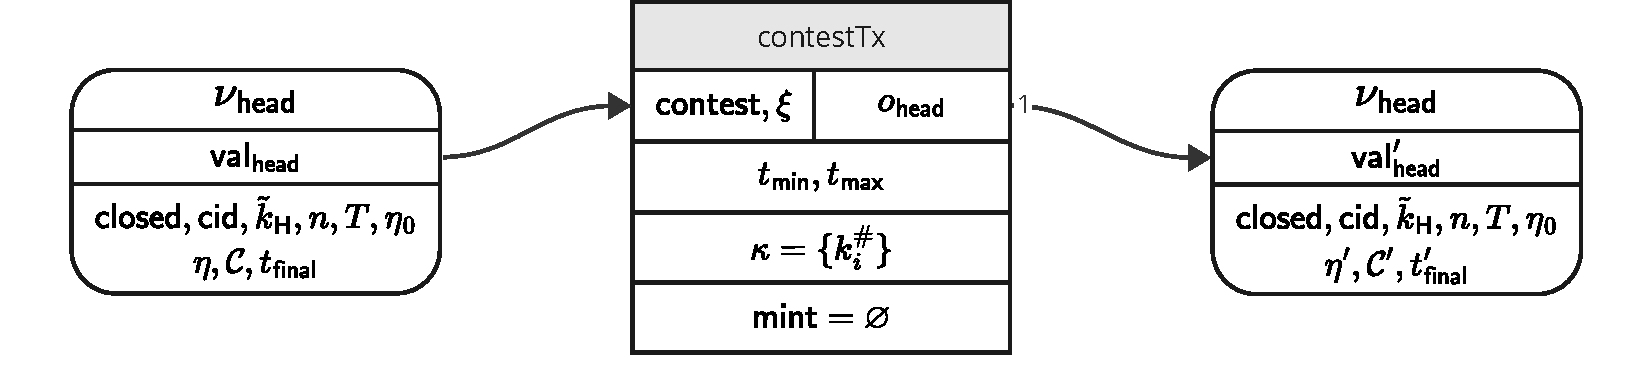
\includegraphics[width=0.8\textwidth]{figures/contestTx.pdf}
	\caption{\mtxContest{} transaction spending the $\stClosed$ head output and producing a different $\stClosed$ head output.}\label{fig:contestTx}
\end{figure}

\subsection{Fan-Out Transaction}

\begin{samepage}
	Once the contestation phase is over, a head may be finalized by posting a
	\mtxFanout{} transaction (see Figure~\ref{fig:fanoutTx}), which
	distributes UTxOs from the head according to the latest state. It consists of
	\begin{itemize}
		\item one input spending from $\nuHead$ holding the $\st$, and
		\item $m$ outputs to fan-out UTxOs.
	\end{itemize}
	Note that \mtxFanout{} represents a final transition of the CEM and hence there
	is no state machine output. The input spending from $\nuHead$ does provide the
	number of fanned-out outputs $m$ as redeemer and checks the state of the CEM is
	advanced to the final $\stFinal$ as follows:
	\[
		(\stClosed,\cid,\hydraKeysAgg,\nop,\cPer,\eta_0,\eta,\contesters,\Tfinal) \xrightarrow[m]{\stFanout} \stFinal,
	\]
\end{samepage}

\noindent The $\nuHead$ validator performs these checks:
\begin{enumerate}
	\item The first $m$ outputs are distributing funds according to
	      $(\cdot, U^{\#}) = \eta$. That is, the outputs correspond (in the same
	      order) to the UTxO canonically combined (see~\ref{sec:collect-tx}) into
	      $U^{\#}$
	      \[
		      \hash(\bigoplus_{j=1}^{m} \bytes(\txOutputs[j])) = U^{\#}
	      \]
	\item Transaction is posted after contestation deadline $\txValidityMin > \Tfinal$
	\item All tokens are burnt
	      $|\{\cid \mapsto \cdot \mapsto -1\} \in \txMint| = n + 1$
\end{enumerate}

\begin{figure}[h]
	\centering
	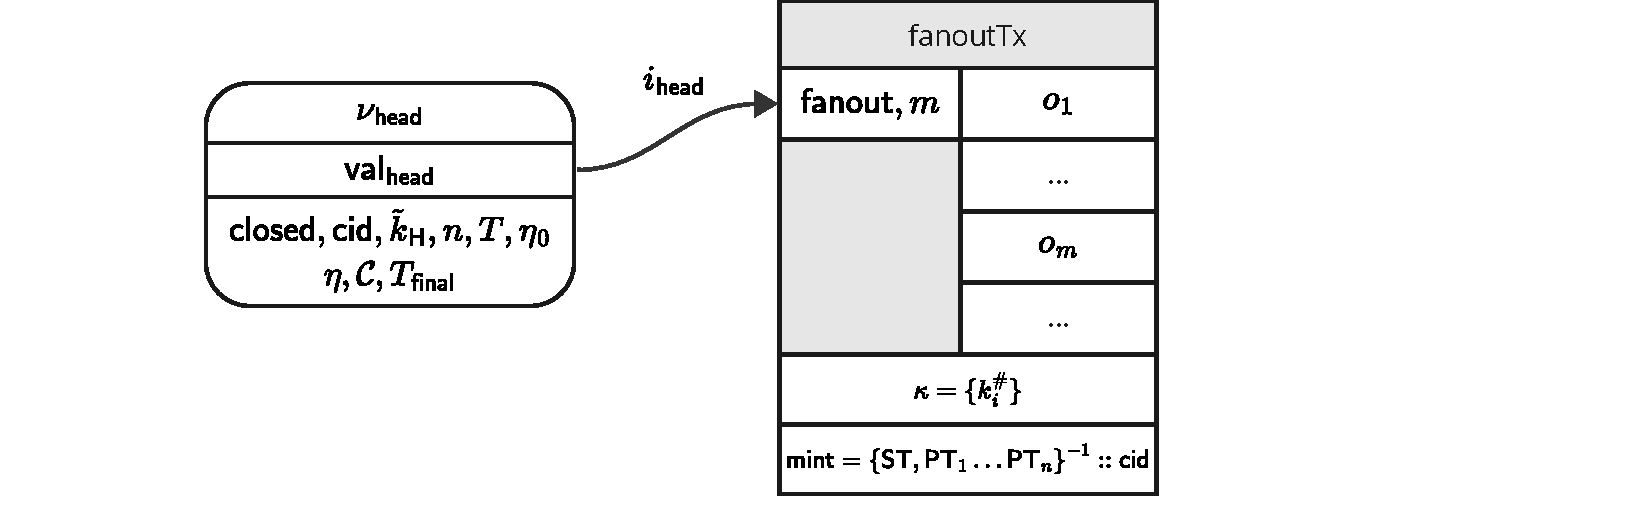
\includegraphics[width=0.8\textwidth]{figures/fanoutTx.pdf}
	\caption{\mtxFanout{} transaction spending the $\stClosed$ head output and
		distributing funds with outputs $o_{1} \dots o_{n}$.}\label{fig:fanoutTx}
\end{figure}

\FloatBarrier{}

%%% Local Variables:
%%% mode: latex
%%% TeX-master: "main"
%%% End:
